%! Suppress = MissingLabel
%! Author = Adrian Helberg
%! Date = 02.02.2020

\documentclass{beamer}
\usetheme{Darmstadt}
% Packages
\usepackage[ngerman]{babel}
\usepackage[utf8]{inputenc}
\usepackage{graphicx}
\usepackage{tikz}

% Meta information
\title{\LARGE{Bachelorprojekt}}
\subtitle{Termin 0}
\author{Adrian Helberg}
\institute{HAW Hamburg \& Hanseaticsoft GmbH}
\date{10.03.2020}
\titlegraphic{
    \begin{picture}
        (0,0)
        \put(-66,206){\makebox(0,0)[rt]{
\includegraphics[width=4cm]{../../resources/Haw_logo.png}}}
        \put(174,200){\makebox(0,0)[rt]{
\includegraphics[width=5cm]{../../resources/Hanseaticsoft_logo.png}}}
    \end{picture}
}

% Document
\begin{document}
    %%% TITLE %%%
    \frame{\titlepage}

    %%% TOC %%%%%
    \frame{
        \frametitle{Inhalt}
        \tableofcontents
    }

    %%% INTRODUCTION


    \section{Einleitung}
    \frame{
        \frametitle{Einleitung}
        \begin{center}
            \begin{tikzpicture}[thick]
                % Nodes
                \node (LR) at (0,0) [rectangle] {
                    
\includegraphics[width=2cm]{../../resources/Lloyds_tile.png}
                };
                \node (HS) at (-4,-4) [rectangle] {
                    
\includegraphics[width=2cm]{../../resources/Hanseaticsoft_tile.png}
                };
                \node (HAW) at (4,-4) [rectangle] {
                    
\includegraphics[width=2cm]{../../resources/Haw_tile.png}
                };
                % Edges
                \draw[->,thick] (LR.south west) -- (HS.north east) node[midway,fill=white] {Partner};
                \draw[<->,thick] (HS.east) -- (HAW.west) node[midway,fill=white] {Kooperation};
            \end{tikzpicture}
        \end{center}
    }

    %%% LLOYDS REGISTER


    \section{Lloyd's Register}
    \frame{
        \frametitle{Lloyd's Register\footnote{\cite{lloyds}{Lloyd's Register}}}
        \begin{picture}
            (0,0)
            \put(0,0){\makebox(320,-50)[rt]{
\includegraphics[width=4cm]{../../resources/Lloyds_logo.png}}}
        \end{picture}
        \begin{itemize}
            \item Schiffs-Klassifikationsgesellschaft
            \item unabhängige Risikomanagement-Organisation
            \item mehr als 9000 Mitarbeiter
            \item in 78 Ländern tätig
            \item Hauptsitz in London
        \end{itemize}
        \\~\\~\\
        \begin{block}{Dienstleistungen}
            \begin{itemize}
                \item Dienstleistungen zur Risikobewertung und -minderung
                \item Zertifizierungen (\textit{Lloyd’s Register Quality Assurance Ltd.})
            \end{itemize}
        \end{block}
    }

    %%% HANSEATICSOFT


    \section{Hanseaticsoft}
    \frame{
        \frametitle{Hanseaticsoft\footnote{\cite{hanseaticsoft}{Hanseaticsoft}}}
        \begin{center}
            
\includegraphics[width=8cm]{../../resources/Hanseaticsoft_logo.png}
        \end{center}
    }

    \subsection{Sitze}
    \frame{
        \frametitle{Sitze\footnote{\cite{hanseaticsoft-contact}{Hanseaticsoft / Contact}}}
        \begin{center}
            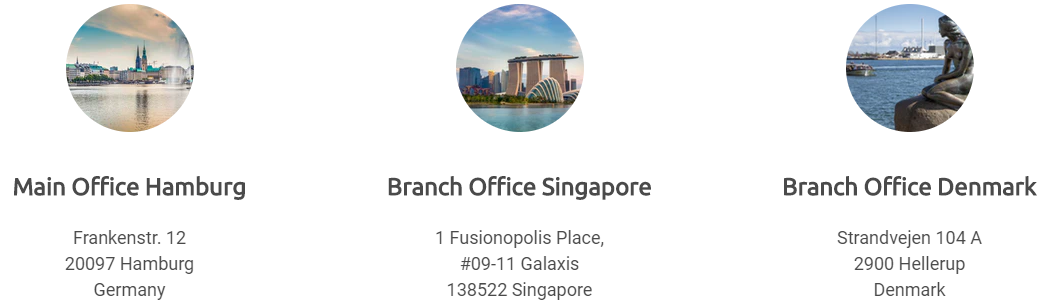
\includegraphics[width=11cm]{../../resources/contact.PNG}
        \end{center}
    }

    \subsection{Kunden}
    \frame{
        \frametitle{Kunden\footnote{\cite{hanseaticsoft-customers}{Hanseaticsoft / Customers}} (5 von 49)}
        \begin{center}
            \begin{tikzpicture}[thick]
                % Nodes
                \node (HS) at (0,0) {
                    
\includegraphics[width=1cm]{../../resources/Hanseaticsoft_tile.png}
                };
                \node (AL) at (0,3) {
                    
\includegraphics[width=2cm]{../../resources/al_logo.png}
                };
                \node (CR) at (3,3) {
                    
\includegraphics[width=2cm]{../../resources/cr_logo.png}
                };
                \node (NH) at (-3,3) {
                    
\includegraphics[width=2cm]{../../resources/nh_logo.png}
                };
                \node (NSC) at (-3,0) {
                    
\includegraphics[width=2cm]{../../resources/nsc_logo.png}
                };
                \node (PTS) at (3,0) {
                    
\includegraphics[width=2cm]{../../resources/pts_logo.png}
                };
                % Edges
                \draw[->,thick] (HS) -- (AL);
                \draw[->,thick] (HS) -- (CR);
                \draw[->,thick] (HS) -- (NH);
                \draw[->,thick] (HS) -- (NSC);
                \draw[->,thick] (HS) -- (PTS);
            \end{tikzpicture}
        \end{center}
    }

    \frame{
        \frametitle{Kunden - Nutzung der Softwarelösungen\footnote{\cite{hanseaticsoft}{Hanseaticsoft / Customers}}}
        \begin{itemize}
            \setlength{\itemsep}{0.4cm}
            \item Organisieren interner Strukturen
            \item Reduzieren von Kommunikationsaufwand und Datentransfer
            \item Ständige Weiterentwicklung von Systemen
            \item Zentrale Bereitstellung von Information
            \item Schaffen von Transparenz
            \item Zentralisierung von Daten
            \item Prozessbeschleunigung
            \item Mobiler Datenzugriff
        \end{itemize}
    }

    \subsection{Dienstleistungen}
    \frame{
        \frametitle{Dienstleistungen\footnote{\cite{hanseaticsoft-solutions}{Hanseaticsoft / Solutions}}}
        \begin{picture}
            (0,0)
            \put(333,64){\makebox(0,0)[rt]{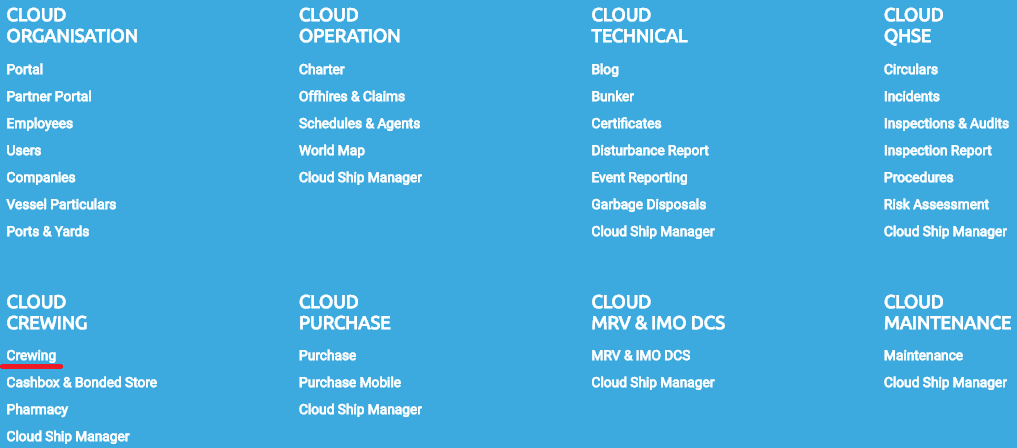
\includegraphics[width=12.6cm]{../../resources/solutions.PNG}}}
        \end{picture}
    }


    \section{Cloud Crewing}
    \frame{
        \frametitle{Cloud Crewing - Crewing\footnote{\cite{crewing}{Hanseaticsof / Cloud Crewing}}}
        \begin{center}
            \begin{tikzpicture}[thick]
                % Nodes
                \node (C) at (-1,0) [rectangle] {
                    
\includegraphics[width=8cm]{../../resources/crewing.png}
                };
                \node (M) at (-4,-4) [rectangle] {
                    Dynamic crew management
                };
                \node (P) at (-0.7,-3) [rectangle] {
                    Cooperative Payroll
                };
                \node (Pl) at (3,-4) [rectangle] {
                    \underline{Detailed planning}
                };
                % Edges
                \draw[->,dashed] (C.south) -- (M.north);
                \draw[->,dashed] (C.south) -- (P.north);
                \draw[->,dashed] (C.south) -- (Pl.north);
            \end{tikzpicture}
        \end{center}
    }

    %%% BIBLIOGRAPHY %%%


    \section{Quellen}
    \frame{
        \frametitle{Quellen}
        \bibliography{main}
        \bibliographystyle{plain}
    }
\end{document}
